\section{Entorno de Desarrollo Local}

Para garantizar la reproducibilidad del proyecto, en esta sección se descibirá el entrono de desarrollo en el que se ha realizado y el acceso al repositorio con el código fuente.

\subsection{Tecnologías y Versiones}

El proyecto se ha desarrollado en un entorno \textbf{Windows 10}, aunque esto no influye en la compatibilidad, ya que todas las tecnologías utilizadas son multiplataforma, lo cual permite realizar el desarrollo en cualquier sistema operativo sin restricciones. En la tabla \ref{tab:dependencias_versiones} se presentan las tecnologías principales empleadas en el proyecto junto con sus versiones correspondientes.

\begin{table}[htbp]
    \centering
    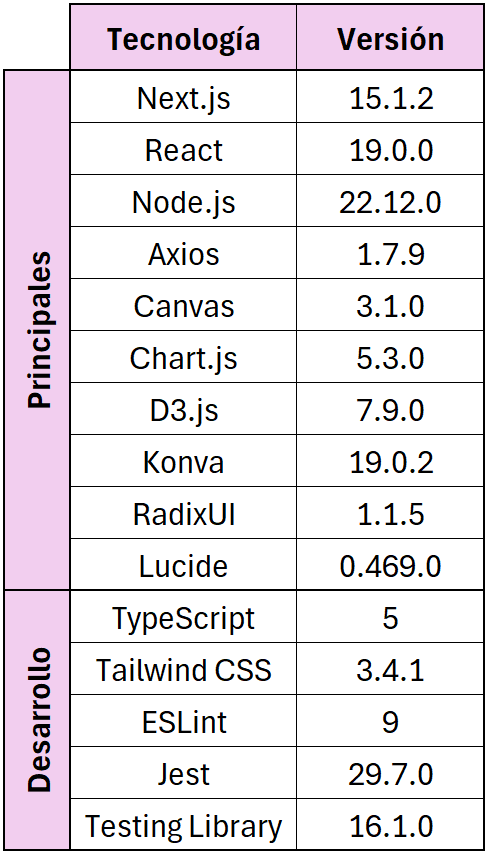
\includegraphics[width=0.37\textwidth]{figures/dependencias_versiones.png}
    \captionsetup{skip=5pt}
    \caption{Dependencias usadas en el desarrollo, junto con sus versiones.}
    \label{tab:dependencias_versiones}
\end{table}

Cabe destacar que el gestor de paquetes utilizado en el proyecto ha sido \textbf{\texttt{pnpm} (\textit{Performant Node Package Manager})}, en lugar de \texttt{npm} (\textit{Node Package Manager}) o \texttt{yarn} (\textit{Yet Another Resource Negotiator}). La elección de \texttt{pnpm} se debe a sus mejoras en la gestión de dependencias y optimización del uso del espacio de almacenamiento. A diferencia de \texttt{npm}, \texttt{pnpm} utiliza un sistema de enlaces en lugar de duplicar archivos en cada proyecto, lo que reduce significativamente el consumo de espacio. Además, \texttt{pnpm} es completamente compatible con los paquetes del registro de \texttt{npm}, lo que garantiza su interoperabilidad con la mayoría de los ecosistemas de desarrollo basados en \textit{Node.js}.

\subsection{Instalación y Configuración del Proyecto}

El proyecto se encuentra alojado en un repositorio de \textit{GitHub}\footnote{Repositorio del proyecto: \href{https://github.com/jonortega/tfg-app-spotify}{https://github.com/jonortega/tfg-app-spotify}} para evitar pérdidas y tener disponibilidad completa al código. Para ejecutarlo localmente, además de haber instalado \textit{Node.js}, hay que clonar el respositorio, acceder a la carpeta y ejecutar los comandos de instalación y ejecución. A continuación, se muestran los comandos necesarios para realizar estos pasos:

\begin{ifalgorithm}[H]
    \begin{lstlisting}[language=bash]
    # Clonar el repositorio
    git clone https://github.com/jonortega/tfg-app-spotify.git
    
    # Acceder al directorio del proyecto
    cd tfg-app-spotify
    
    # Instalar dependencias
    pnpm install
    
    # Ejecutar el servidor de desarrollo
    pnpm run dev
    \end{lstlisting}
    \caption{Comandos de instalación y ejecución inicial del proyecto.}
    \label{alg:instalacion_proyecto}
\end{ifalgorithm}

Tras estos pasos, la página web estará accesible en \texttt{localhost:3000}. Es encesario agregar un fichero de variables de entorno \texttt{.env.local}, ya que, por seguridad, no se registra en el sistema de control de versiones. El contenido de dicho fichero se muestra en el \hyperref[ch:anexoC]{Anexo C} (algoritmo \ref{alg:variables_entorno}).

Dos de las variables de entorno necesarias para poder tratar con la API de \textit{Spotify}, son el \textbf{Client ID} y el \textbf{Client Secret}. Estos dos valores se obtienen al realizar el registro de la aplicación en la plataforma de desarrollo de \textit{Spotify}. En la siguiente sección, se explicará cómo realizar este registro y dónde obtener dichas variables.

\newpage

\section{Registro de la Aplicación en Spotify}

Para poder obtener datos de la Web API de \textit{Spotify}, es necesario registra la aplicación en su plataforma de desarrollo\footnote{Spotify for Developers: \href{https://developer.spotify.com/}{https://developer.spotify.com/}}. Tras inciar con una cuenta, se nos presentará un panel donde podremos crear una nueva app. \textit{Spotify} pedirá algunos datos (figura \ref{fig:create_app}), que tendremos que rellenar. Los campos como \textit{Redirect URIs} pueden ser modificados posteriormente, ya que tendremos que actualizarlo con el dominio indicado tras el despliegue de la aplicación.

\begin{figure}[H]
    \centering
    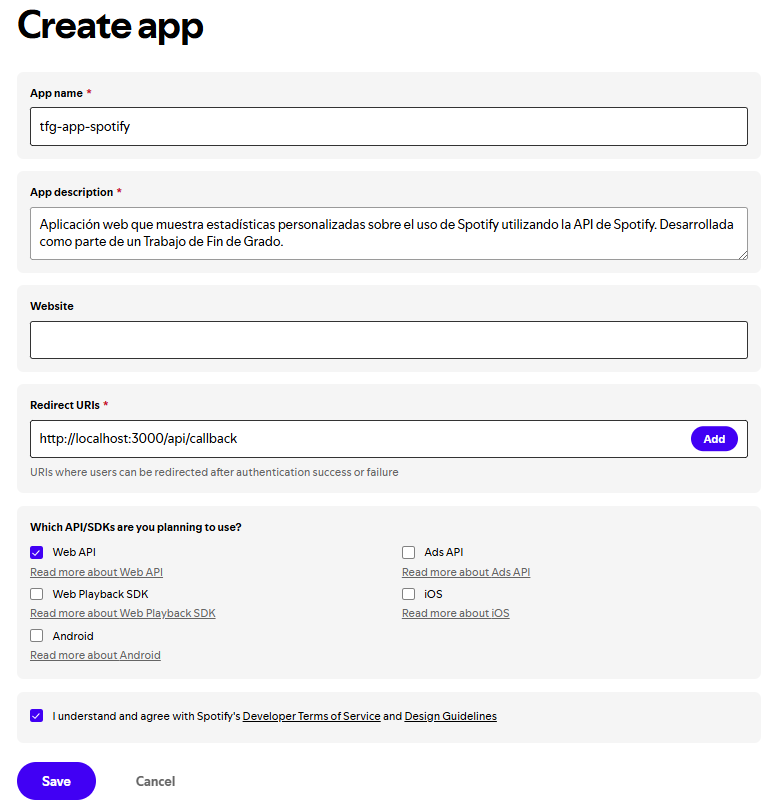
\includegraphics[width=0.65\textwidth]{figures/registro_spotify/create_app.png}
    \caption{Panel de creación de app en la plataforma de \textit{Spotify}.}
    \label{fig:create_app}
\end{figure}

Al aceptar los términos y crear la app, tendremos acceso al \textit{Client ID} y \textit{Client Secret}. Estos se encuentran en los ajustes (\textit{settings}) y tendremos que expandir el panel para poder ver los dos valores (figura \ref{fig:client_id_secret}).

\begin{figure}[H]
    \centering
    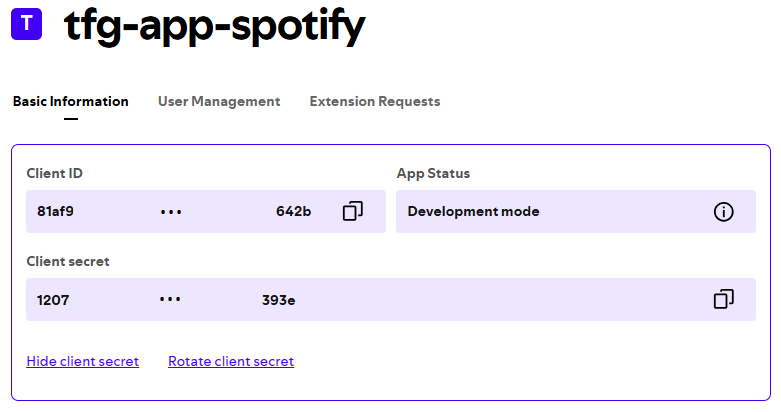
\includegraphics[width=0.65\textwidth]{figures/registro_spotify/client_id_secret.png}
    \caption{Panel de ajustes con el \textit{Client ID} y el \textit{Client Secret}.}
    \label{fig:client_id_secret}
\end{figure}

En el caso en el que el \textit{Client Secret} haya sido comprometido, es posible generar uno nuevo, anulando el anterior y evitando tener que desechar la aplicación registrada. También se muestra un campo llamado \textit{App Status} con el valor \textbf{Development Mode}. Esto significa que la aplicación registrada está en ``desarrollo'', por lo que existen las siguientes restricciones:

\begin{itemize}
    \item Un máximo de 25 usuarios (cuentas verificadas de \textit{Spotify}) pueden usar la aplicación.
    \item Cada usuario tiene que estar registrado en una lista de permitidos (\textit{allowlist}) de la plataforma.
\end{itemize}

Es posible eliminar estas restricciones, enviando una solicitud a \textit{Spotify} para cambiar el estado de \textit{Development Mode} a \textbf{Extended Quota Mode}. En el caso de que sea aceptada, se elimina cualquier restricción sobre el número de usuarios permitidos y no será necesario registrarlos anteriormente, además de ampliar el umbral de la tasa de peticiones (\textit{rate limit}). En este trabajo \textbf{no se va a realizar dicha solicitud}, por lo que tendremos que acogernos a las limitaciones impuestas en el modo de desarrollo. Esto requiere que se registren las cuentas de usuarios que vayan a probar la aplicación en la pestaña de gestión de usuarios (figura \ref{fig:user_management}).

\begin{figure}[H]
    \centering
    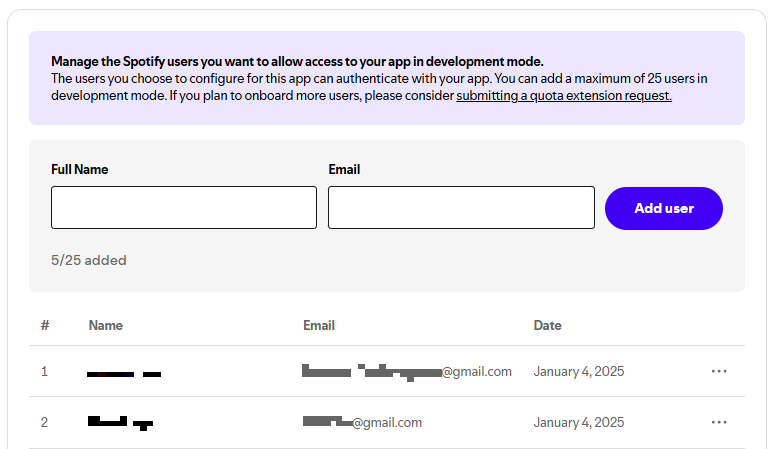
\includegraphics[width=0.75\textwidth]{figures/registro_spotify/user_management.png}
    \caption{Panel de gestión de usuarios que tienen acceso a la aplicación.}
    \label{fig:user_management}
\end{figure}

Con estos pasos, se habrá realizado correctamente el registro de la aplicación y obtención del \textit{Client ID/Secret}, imprescindibles para la comunicación con la API de \textit{Spotify}. En la plataforma de desarrollo, además, tenemos accesible un panel para poder monitorear la actividad de la aplicación (\hyperref[ch:anexoC]{Anexo C}, figura \ref{fig:dashboard_spotify}).

\section{Ciclo de Vida del Desarrollo}

\subsection{Incremento I: Prototipado Rápido}

\subsection{Incremento II: Producto Mínimo Viable (PMV)}

\subsection{Incremento III: Producto Final}

\section{Implementación del Fronted}

\subsection{Lógica de las Estadísticas}

\subsection{React Hooks}

\section{Implementación del Backend}

\subsection{Lógica y Tratamiento de Datos en el Servidor}

\subsection{Estructuras de Datos}

\section{Optimizaciones}